\documentclass[border=3pt]{standalone}
% Preâmbulo compartilhado pelos diagramas TikZ da aula 8 de IHR (Métodos de Pesquisa)
\usepackage[T1]{fontenc}
\usepackage[utf8]{inputenc}
\usepackage{lmodern}
\usepackage{amsmath}
\usepackage{xcolor}
\usepackage{tikz}
\usetikzlibrary{arrows.meta,angles,quotes,decorations.pathmorphing,decorations.pathreplacing,calc,
                positioning,shapes.geometric,shapes.misc,backgrounds,fit,
                math}

% Paleta (mesma dos SVGs originais)
% Paleta da disciplina de IHR: acento azul (#1A6FB5), cor de destaque do tema.
% (o nome "dblue" é mantido para não alterar todos os diagramas)
\definecolor{dblue}{HTML}{1A6FB5}
\definecolor{dorange}{HTML}{B3541E}
\definecolor{dgreen}{HTML}{4A7C59}
\definecolor{dred}{HTML}{9C4B4B}
\definecolor{dcream}{HTML}{F4F1EA}
\definecolor{dshade}{HTML}{DDD7C9}

% Função gaussiana (não normalizada por padrão de escala visual)
\pgfmathdeclarefunction{gauss}{3}{%
  \pgfmathparse{1/(#3*sqrt(2*pi))*exp(-((#1-#2)^2)/(2*#3^2))}%
}

% Estilos comuns (prefixo d... para não colidir com chaves internas do pgf)
\tikzset{
  >={Stealth[length=2mm]},
  dguide/.style={gray!55, dashed, line width=0.4pt},
  daxis/.style={gray!60, line width=0.7pt, ->},
  dbody/.style={fill=black!3, draw=black!80, line width=1pt},
  dacc/.style={draw=dblue, line width=1pt},
  dlbl/.style={black!55, font=\small},
  dsub/.style={black!45, font=\footnotesize},
  dstate/.style={circle, draw=black!80, fill=dcream, line width=1pt,
                 minimum size=17mm, font=\large, inner sep=1pt},
  dobs/.style={circle, draw=black!80, fill=dshade, line width=1pt,
               minimum size=14mm, font=\large, inner sep=1pt},
  dbox/.style={rounded corners=2pt, draw=black!80, fill=dcream, line width=1pt,
               align=center, inner sep=6pt},
  dop/.style={circle, draw=black!80, fill=white, line width=1pt,
              minimum size=6mm, inner sep=0pt, font=\small},
  dtrans/.style={->, dblue, line width=1pt},
  dmeas/.style={->, dorange, line width=1pt},
  dcurve/.style={line width=1pt, dblue},
  dcurveb/.style={line width=1.4pt, dorange},
}

\begin{document}
\hyphenpenalty=10000 \exhyphenpenalty=10000 \tolerance=9999 \emergencystretch=3em
\newcommand{\rob}[2]{% x, y
  \draw[dgreen, fill=dgreen!15, line width=1.4pt, rounded corners=3pt] (#1-0.5,#2-0.1) rectangle (#1+0.5,#2+0.8);
  \fill[dgreen] (#1-0.19,#2+0.45) circle (0.08); \fill[dgreen] (#1+0.19,#2+0.45) circle (0.08);
  \draw[dgreen, line width=1.3pt] (#1,#2+0.8) -- (#1,#2+1.1); \fill[dgreen] (#1,#2+1.18) circle (0.07);
  \draw[dgreen, fill=dgreen!15, line width=1.4pt, rounded corners=4pt] (#1-0.6,#2-0.95) rectangle (#1+0.6,#2-0.25);}
\newcommand{\pess}[2]{% x, y
  \draw[dblue, fill=dblue!15, line width=1.3pt] (#1,#2+0.36) circle (0.24);
  \draw[dblue, fill=dblue!15, line width=1.3pt, rounded corners=4pt] (#1-0.42,#2-0.55) rectangle (#1+0.42,#2+0.05);}
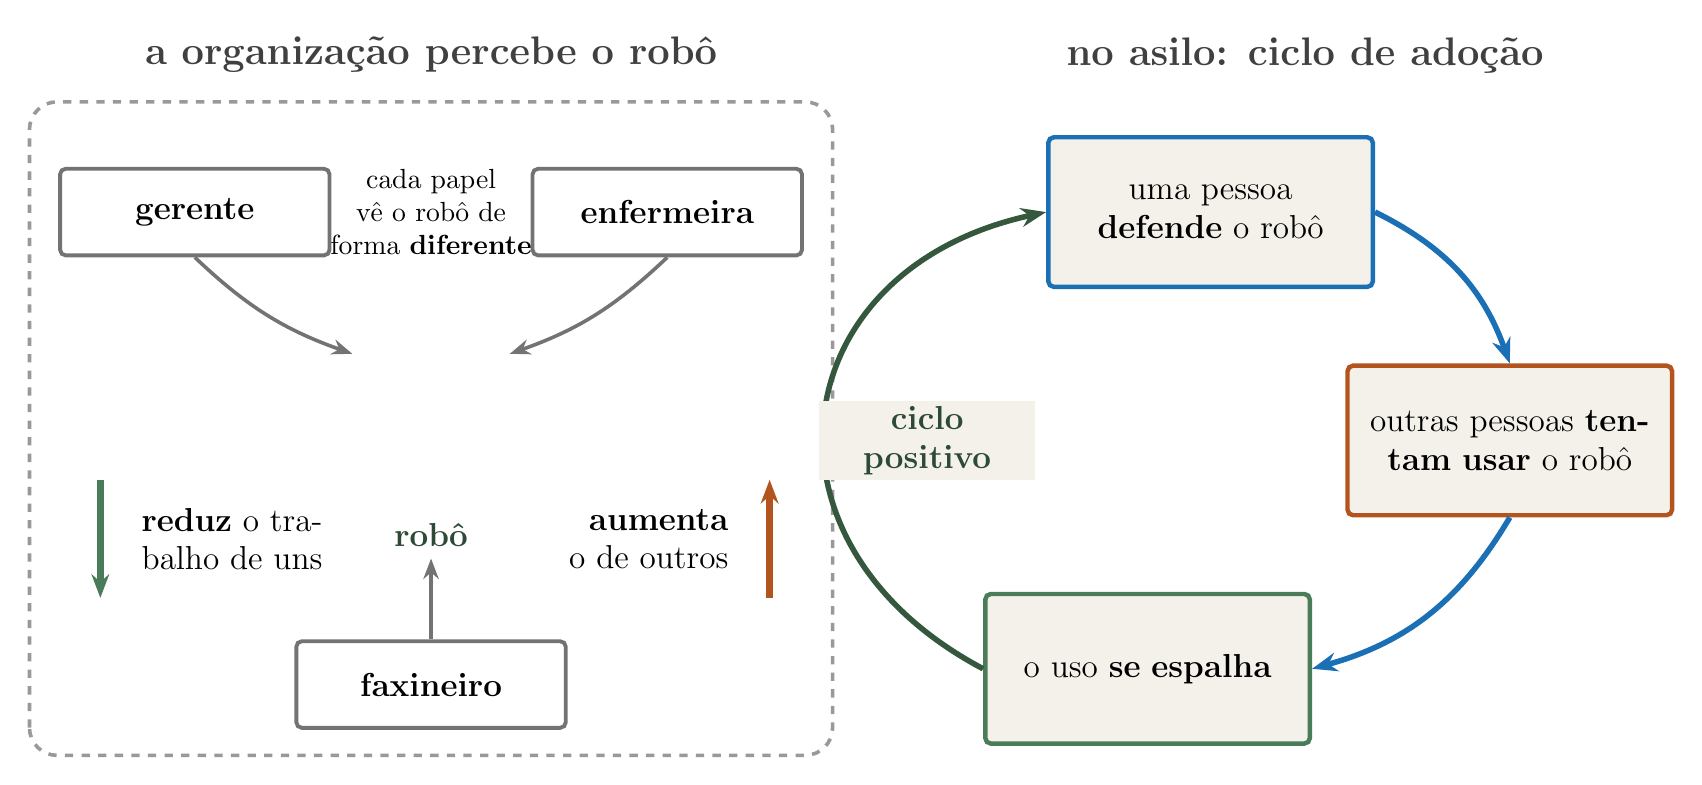
\begin{tikzpicture}[x=1cm,y=1cm]
  \tikzset{role/.style={dbox, draw=black!55, fill=white, line width=1.4pt, text width=3.0cm, minimum height=1.1cm, font=\large\bfseries, align=center},
           nd/.style={dbox, line width=1.6pt, text width=3.7cm, minimum height=1.9cm, font=\large, align=center}}
  % ---------- painel esquerdo: papéis ----------
  \node[font=\Large\bfseries, black!75] at (4.9,9.3) {a organização percebe o robô};
  \draw[black!40, dashed, line width=1.3pt, rounded corners=10pt] (-0.2,0.4) rectangle (10.0,8.7);
  \rob{4.9}{4.6}
  \node[font=\large\bfseries, dgreen!60!black] at (4.9,3.2) {robô};
  \node[role] (g) at (1.9,7.3) {gerente};
  \node[role] (e) at (7.9,7.3) {enfermeira};
  \node[role] (f) at (4.9,1.3) {faxineiro};
  \draw[black!55, line width=1.3pt, -{Stealth[length=2.6mm]}] (g.south) to[bend right=12] (3.9,5.5);
  \draw[black!55, line width=1.3pt, -{Stealth[length=2.6mm]}] (e.south) to[bend left=12] (5.9,5.5);
  \draw[black!55, line width=1.3pt, -{Stealth[length=2.6mm]}] (f.north) -- (4.9,2.9);
  \node[font=\normalsize, text width=2.9cm, align=center] at (4.9,7.3) {cada papel vê o robô de forma \textbf{diferente}};
  % trabalho
  \draw[dgreen, line width=2.6pt, -{Stealth[length=3mm]}] (0.7,3.9) -- (0.7,2.4);
  \node[font=\large, anchor=west, text width=2.7cm] at (1.1,3.15) {\textbf{reduz} o trabalho de uns};
  \draw[dorange, line width=2.6pt, -{Stealth[length=3mm]}] (9.2,2.4) -- (9.2,3.9);
  \node[font=\large, anchor=east, text width=2.6cm, align=right] at (8.8,3.15) {\textbf{aumenta} o de outros};
  % ---------- painel direito: ciclo de adoção ----------
  \node[font=\Large\bfseries, black!75] at (16.0,9.3) {no asilo: ciclo de adoção};
  \node[nd, draw=dblue] (a) at (14.8,7.3) {uma pessoa \textbf{defende} o robô};
  \pess{12.2}{7.3}
  \node[nd, draw=dorange] (b) at (18.6,4.4) {outras pessoas \textbf{tentam usar} o robô};
  \node[nd, draw=dgreen] (c) at (14.0,1.5) {o uso \textbf{se espalha}};
  \draw[dtrans, line width=2pt, -{Stealth[length=3.2mm]}] (a.east) to[bend left=22] (b.north);
  \draw[dtrans, line width=2pt, -{Stealth[length=3.2mm]}] (b.south) to[bend left=22] (c.east);
  \draw[dgreen!70!black, line width=2pt, -{Stealth[length=3.2mm]}] (c.west) to[bend left=70, looseness=1.5] (a.west);
  \node[font=\large\bfseries, dgreen!60!black, text width=2.6cm, align=center, fill=dcream, inner sep=2pt] at (11.2,4.4) {\textbf{ciclo positivo}};
\end{tikzpicture}
\end{document}
